%!TEX root = main.tex

\chapter{Fourier Transform}
\label{Fourier Transformation}

\begin{figure}[H]
	\begin{center}
		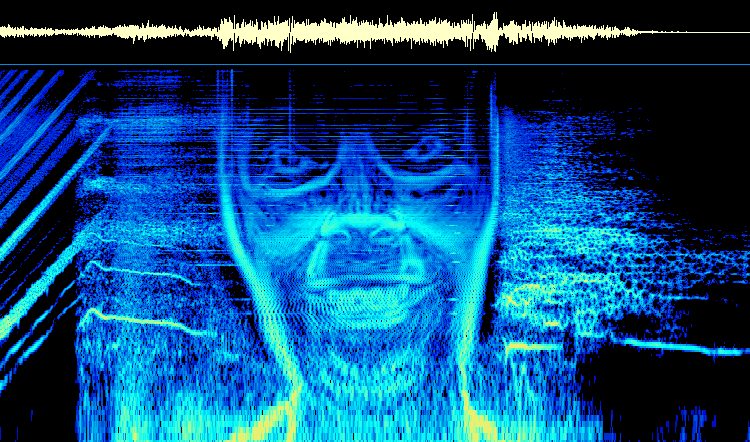
\includegraphics[width = 14cm]{img/aphexFFT.png}
		\caption{Image in the spectrogram in a track by ``Aphex Twin''.}
		\label{fig:Aphex}
	\end{center}
\end{figure}




\begin{center}
\begin{figure}[H]
\tikzset{concept/.append style={fill={none}}}
\begin{tikzpicture}
  \path[mindmap,concept color=black,text=black]
	node[concept] {Fourier Tansform}
	[clockwise from=0]
	% child[concept color=green!50!black] {
	% node[concept] {schuluebung v. letzem Mal}
	% }
	% child[concept color=green!50!black] {node[concept] {pd parxis}
	% 	child[concept color=green!50!black] {node[concept] {send/receive}}
	% 	child[concept color=green!50!black] {node[concept] {initialisierung}}
	% 	}
	% child[concept color=blue] {
	% node[concept] {hauptteil FFT}
	% [clockwise from=-90]
		child[concept color=orange] { node[concept] {theory} }
		child[concept color=red] { node[concept] {practice}
			child[concept color=red] { node[concept] {spectrum display} }
			child[concept color=red] { node[concept] {fft filter}
				child[concept color=red] { node[concept] {random filter} }
				}
			child[concept color=red] { node[concept] {fft reverb} }
			child[concept color=red] { node[concept] {pitch shift} }
		}


;
\end{tikzpicture}
\caption{Lecture Contents: Fourier Transform}
\end{figure}
\end{center}

\section{Further Information}

\begin{itemize}
	\item \link{https://www.youtube.com/watch?v=-IJuqR6nz\_Q}{complex Numbers}
	\item \link{https://www.youtube.com/watch?v=EIstpPXKWng}{The Imaginary Number}
	\item \link{http://jackschaedler.github.io/circles-sines-signals}{Interactive Visualization of the Fourier Transform}

\end{itemize}

% vorbereitung:\\
% Eulers identity, complex numbers.



% Initialisierung
% Fourier transformation.
% Spectral filter
% Spectral Reverb, delay.
% Windowing
% Convolution,
% evtl. cross correlation
% freq. crossover
% spectral synyth,
% spectraum display.


% evtl auch:
% \begin{itemize}
% 	\item send / receive, send / receive bei gui objekten.
% 	\item initialisierung
% 	\item
% \end{itemize}


% Diskretes Signal -> Periodisches Spectrum \\
% Periodisches Signal -> Diskretes Spectrum



% fftuebung
% beiwerk:
	% initialisierung
	% send/receive
% schuluebung von letzem mal
% hauttteil fft
	% theorie	> geschichte
	% praxis
		% spectrum display
		% fft filter
			% nomral
			% random
		% fftdelay
		% fft reverb
		% pitch shift


% \section{Fourier Transformation}
\section{Concept}
The Fourier transform is a way to switch domains. What does that mean? We can think of it as transforming a piece of information into another representation without loss of information. To give an analogy: \\
If I tell you, we meet at \textit{Matthias Corvinus-Straße 15, 3100 St. Pölten} it is the same as telling you we meet at GPS coordinates 48.2138731, 15.6320195. It is the same information in another format, another \textit{domain}.\\
These two formats have different advantages and disadvantages. For example, would you know if the location in GSP format is even in Austria? Probably not. On the other hand, in which direction (north, south, east, west) do I have to go from the FH to get to the main train station? easy to see GPS: the main train station is at 48.20850,15.62515. Both numbers are lower so it must be south west. Not so easy to see if I tell you the train station is at Bahnhofplatz 1,3100 St. Pölten. \\
The point is, depending on what we want, different representations offer different possibilities and insights.
\begin{figure}[H]
	\centering
	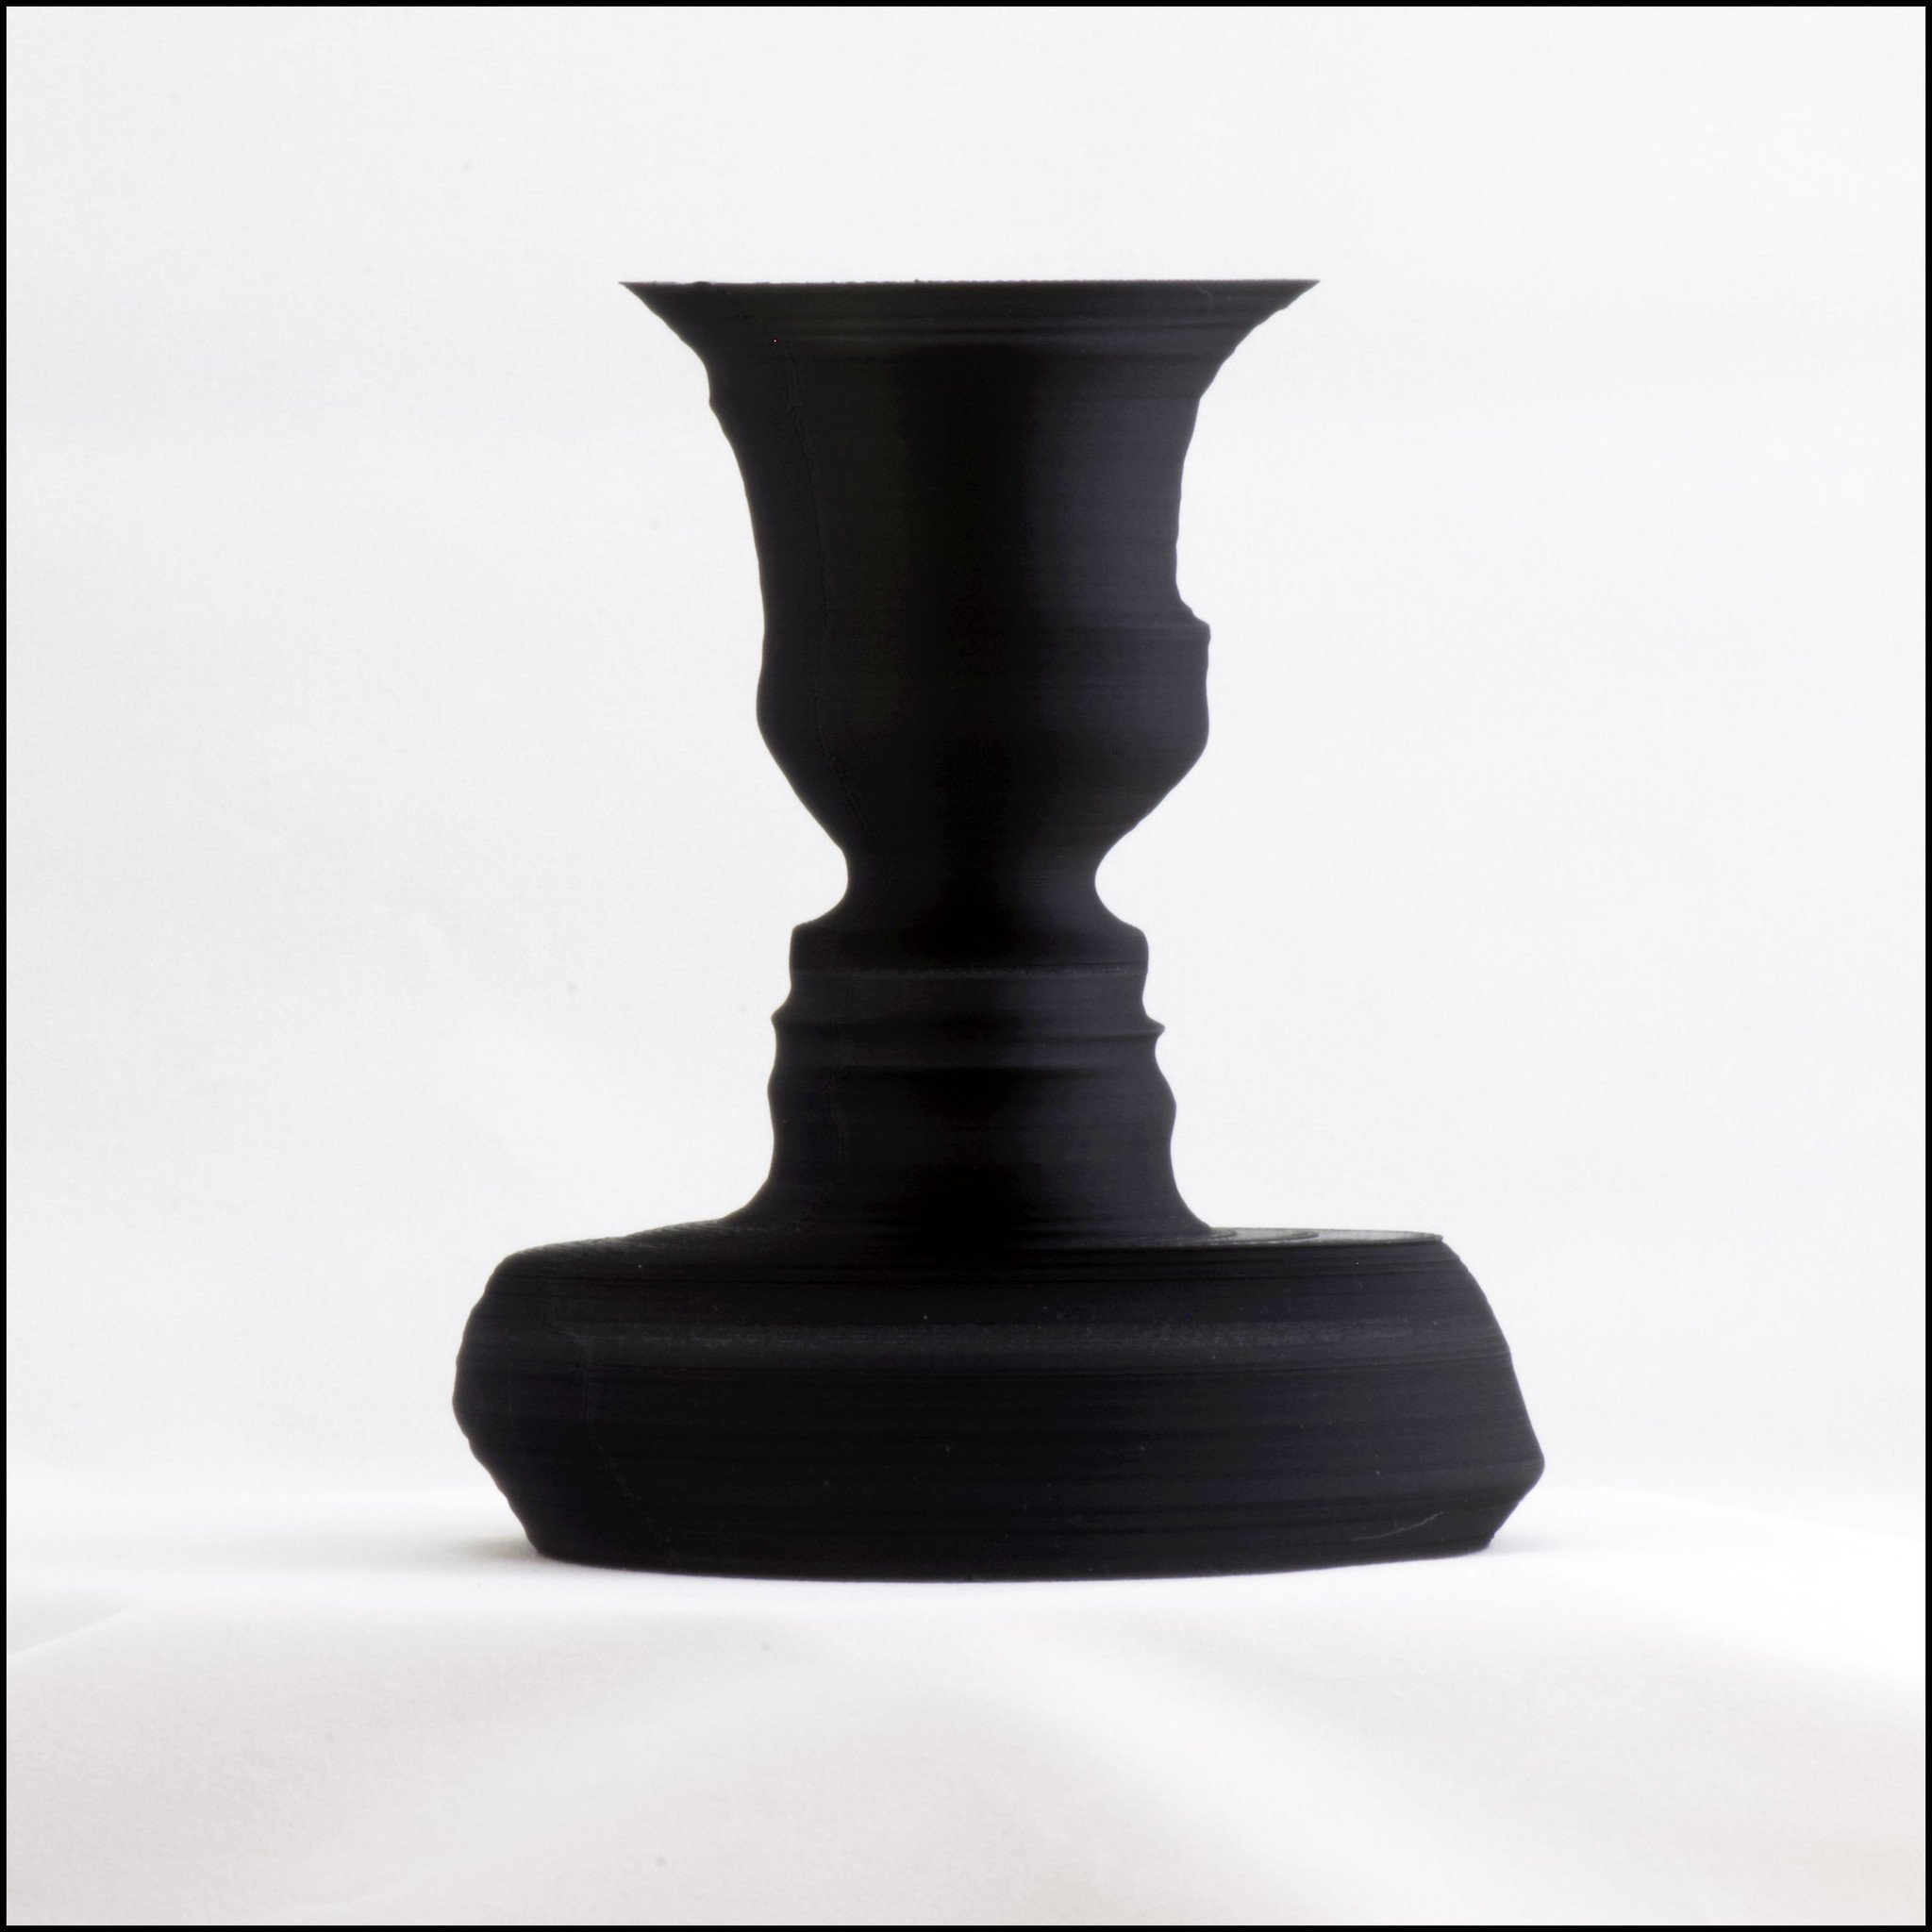
\includegraphics[width=\textwidth]{img/vase.jpg}
	\caption[illusion]
	{Depending on how you look at something, different possibilities and insights arise.}
	\label{fig:vase}
\end{figure}

In the case of the Fourier transform we want to switch to a spectral domain. We want to do this since it would enable us to immediately see if there is a lot of energy at a certain frequency. Oddly, with light in the physical world, this seems very simple, just take a prism:

\begin{figure}[H]
	\centering
	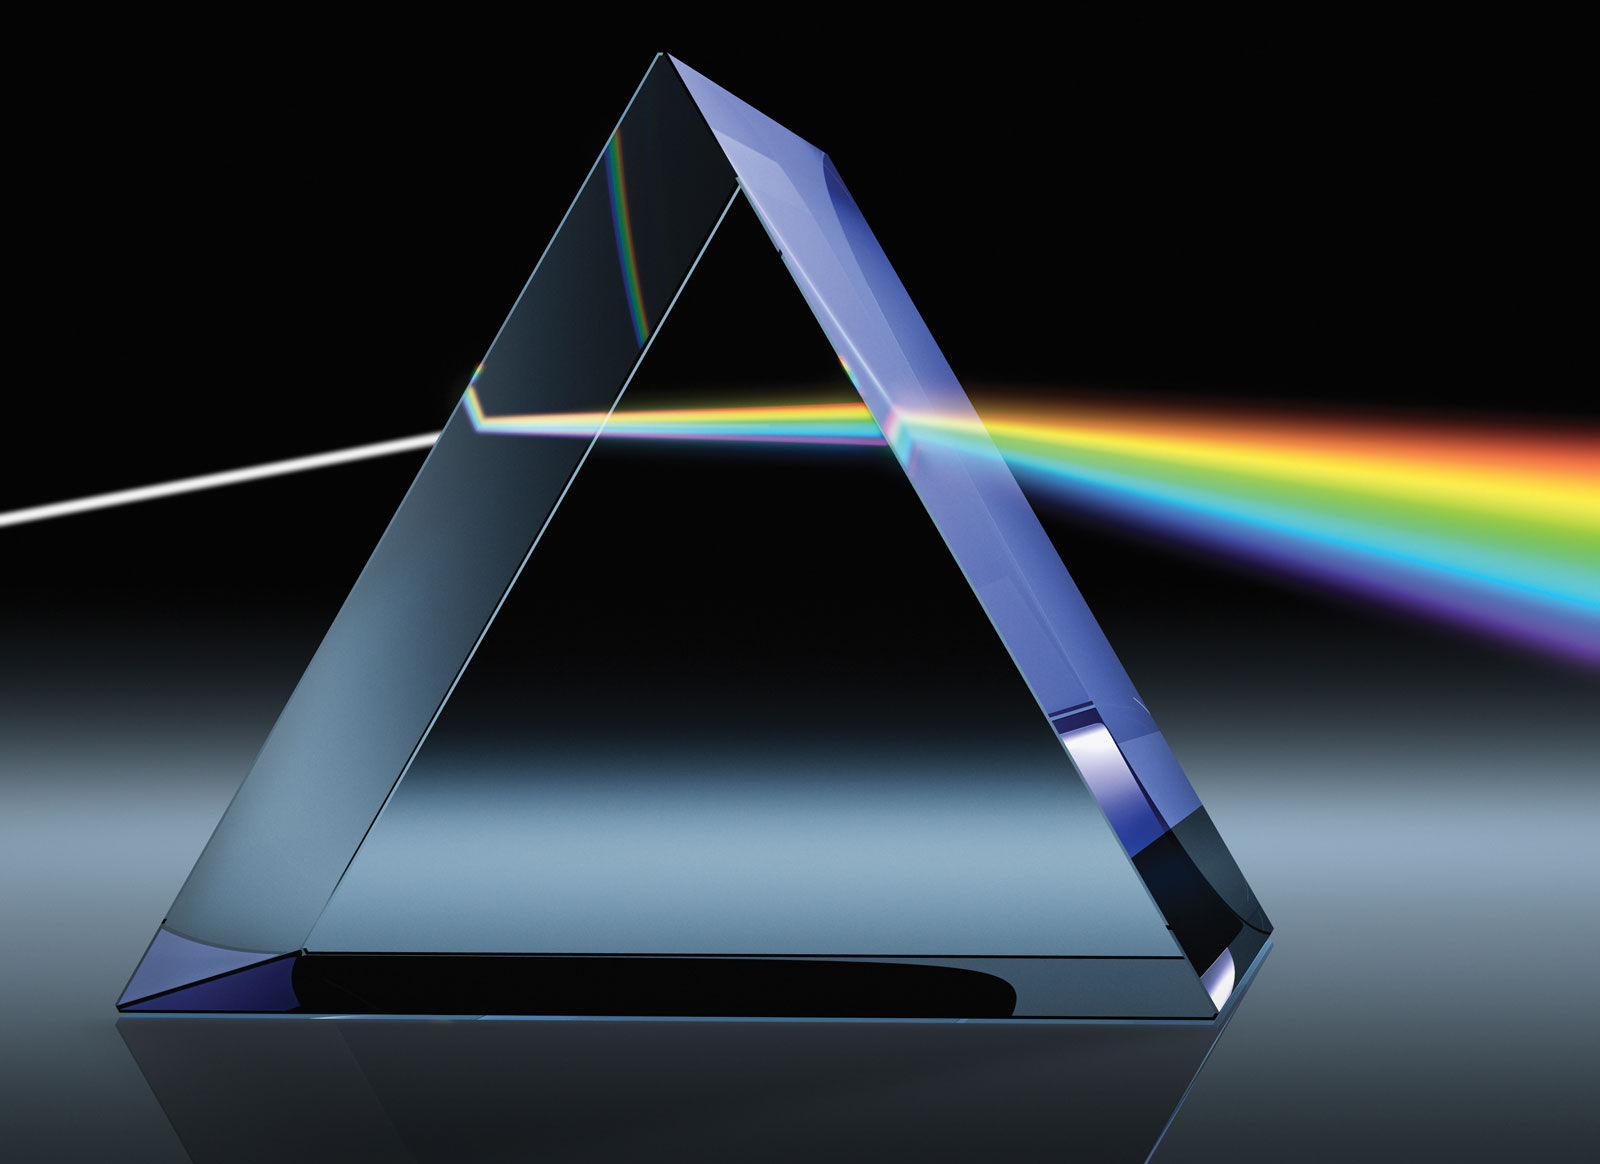
\includegraphics[width=\textwidth]{img/Prism.jpg}
	\caption[prism]
	{A prism splits up light into its different spectral components, essentially performing a Fourier transform.}
	\label{fig:prism}
\end{figure}

\section{Math}
So how do we do this domain switching? There are different approaches to explaining what's happening in the Fourier Transform, but I think this is the most intuitive one: Remember, we just want to know how much of a certain frequency is contained in a certain signal $x(t)$.\\
If I give you 100 Euros and ask you to tell me how many 5 Euro bills are "in there", what would you do? Divide, of course. So can we just take a time domain signal and divide it by a sine at some frequency to see how much of it is contained in that signal? Yes!\\
The Fourier transform is defined as

\begin{equation}
	X(f)= \mathcal{F} \{x(t)\} = \int_{-\infty}^\infty \! x(t) e^{-i2\pi ft} \, \mathrm{d}t
	\label{ft}
\end{equation}

Most of the time we are dealing with discrete (digital) signals, but since the  \textit{Discrete Fourier Transform} (DFT) is a bit less intuitive, let's stick to the continuous('analog') one.


What does Equation \ref{ft} mean? We have an input time domain signal $x(t)$. We get out a frequency domain signal $X(f)$. In order to see why this is working, we need to remember Euler's identity:

\begin{equation}
	e ^{ix} = cos(x)+i \cdot sin(x)
\end{equation}

So, the Fourier transform actually is an integral (a continuous summation) over the input signal times cosine and sine terms:


\begin{equation}
	X(f)= \mathcal{F} \{x(t)\} = \int_{-\infty}^\infty \! x(t) \cdot (cos(2\pi ft)+i \cdot sin(2\pi ft) )^{-1}  \, \mathrm{d}t
	\label{ft2}
\end{equation}

And, knowing that a negative exponent means the same as using the reciprocal, so dividing, we can rearrange to:


\begin{equation}
	X(f)= \mathcal{F} \{x(t)\} = \int_{-\infty}^\infty \! \frac{x(t)} { cos(2\pi ft)+i \cdot sin(2\pi ft) }  \, \mathrm{d}t
	\label{ft2}
\end{equation}

Now you can probably see that we just take the input signal, and for each frequency $f$, we just "sum" over the whole input signal to see how much sine and cosine of that frequency is contained. Ok, it's complex sinusoids, we didn't touch on complex numbers etc, but this should give you a feeling why this can work.

% \begin{equation}
% 	x_f(m) = \sum_{n=0}^{N-1} x(n)\cdot (cos(2 \pi \frac{n m}{N})+i \cdot sin(2 \pi \frac{n m}{N}))^{-1}
% \end{equation}


For the sake of completeness, here are some variants of the whole scheme:\\
% Geschichte:
% Bernoulli, Euler, Gauß, Fourier
The discrete Fourier Transform (DFT) is defined as:
\begin{equation}
	x_f(m) = \sum_{n=0}^{N-1} x(n)\cdot e^{-i 2 \pi \frac{n m}{N} }
	\label{eq:dft}
\end{equation}


Inverse Fourier Transformation:\\
\begin{equation}
	x(t)= \mathcal{F}^{-1} \{X(f)\} = \int_{-\infty}^\infty \! X(f) e^{j2\pi ft} \, \mathrm{d}f
\end{equation}

\section{Implementation}


As python code this could look like the following. Please refer to Equation \ref{eq:dft}. The code below uses the same variable names to make this as little confusing as possible.
\newpage
\lstinputlisting[language=Python,caption={DFT in python},captionpos=b]{code/fourierTransform.py}
The above code produces the following plot:
\begin{figure}[H]
	\centering
	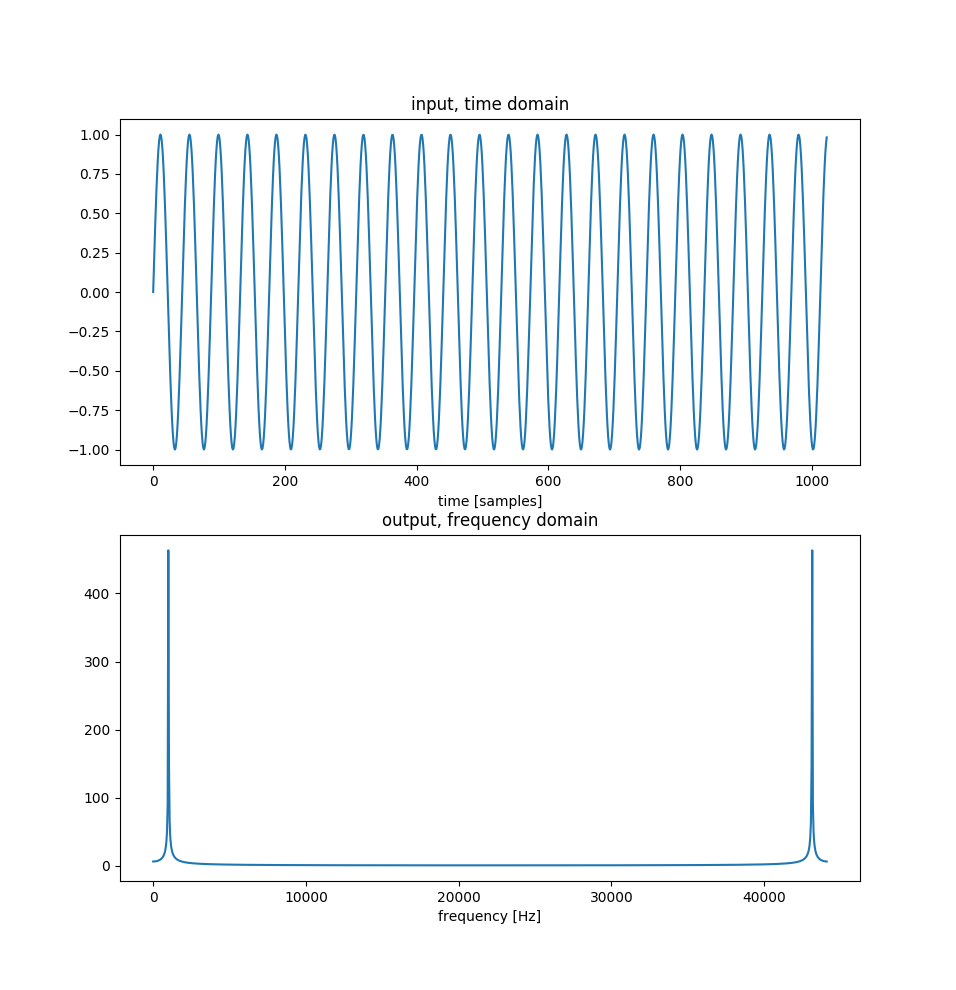
\includegraphics[width=\textwidth]{img/pythonDFT.png}
	\caption[DFT Plot]
	{Plot produced by the script above.}
	\label{fig:pyfft}
\end{figure}

\comm{Note: X axis in fig \ref{fig:pyfft} is wrong! Should go from 0 to 22050 and back to 0.}

Beware that the python code above implements Equation \ref{eq:dft} directly. It is \textit{very} slow. Typically, a different algorithm is used, such as an implementation of the Fast Fourier Transform (FFT). In python, there are several ways to compute an FFT in an efficient way such as \texttt{numpy.fft.fft()}. The FFT is a classic \textit{divide and conquer} solution to performance boosting an algorithm.\\
We need to address something here: We send a single frequency into the DFT and we expect a single spike, showing that we have energy at one frequency. And we get two peaks. This is because the FFT produces a mirrored, a two-sided spectrum. Basically, \textbf{you can ignore half of the plot}. Why is that? The explanation has to do with the fact that digital signals always have an infinite periodic spectrum. You might connect this to the phenomenon of aliasing.

\video{
	In video and image processing, the DFT does not play such a big role as in audio, but the discrete cosine transform does. The differences between the DFT and the DCT are:
	\begin{itemize}
		\item The DCT produces a real output, the DFT a complex one
		% \item The DCT has more resolution in the low-Frequency range
		\item there are several different forms of DCT and there is also the discrete Sine Transform (DST)
		\item The DCT tends to have more energy in its low frequency bins and is therefore more suitable for lossy data-compression (since we throw away high frequency or low energy bins)
	\end{itemize}
	For more information on the DCT and compression have a look at \href{https://www.youtube.com/watch?v=Q2aEzeMDHMA}{Jpeg compression and the discrete Cosine Transform}\footnotemark
}
\footnotetext{https://www.youtube.com/watch?v=Q2aEzeMDHMA}
\section{Application in pd}
We won't code a DFT in pd. Probably it's possible but didactically it wouldn't be very helpful and practically it would be a pita\footnote{Certain kind of bread.}. But we need to know how to use the FFT in pd. There are 4 objects of particular interest here:
\begin{itemize}
	\item \pd{fft\textasciitilde} fast (discrete) fourier transform
	\item \pd{ifft\textasciitilde} fast (discrete) inverse fourier transform
	\item \pd{rfft\textasciitilde} fast (discrete) fourier transform, real only
	\item \pd{rifft\textasciitilde} fast (discrete) inverse fourier transform, real only
\end{itemize}
The 'real only' versions assume that our time domain signals are not complex, so have no imaginary component, which is almost always the case.
\subsection{Filtering using the FFT}
\begin{figure}[h]
	\begin{center}
		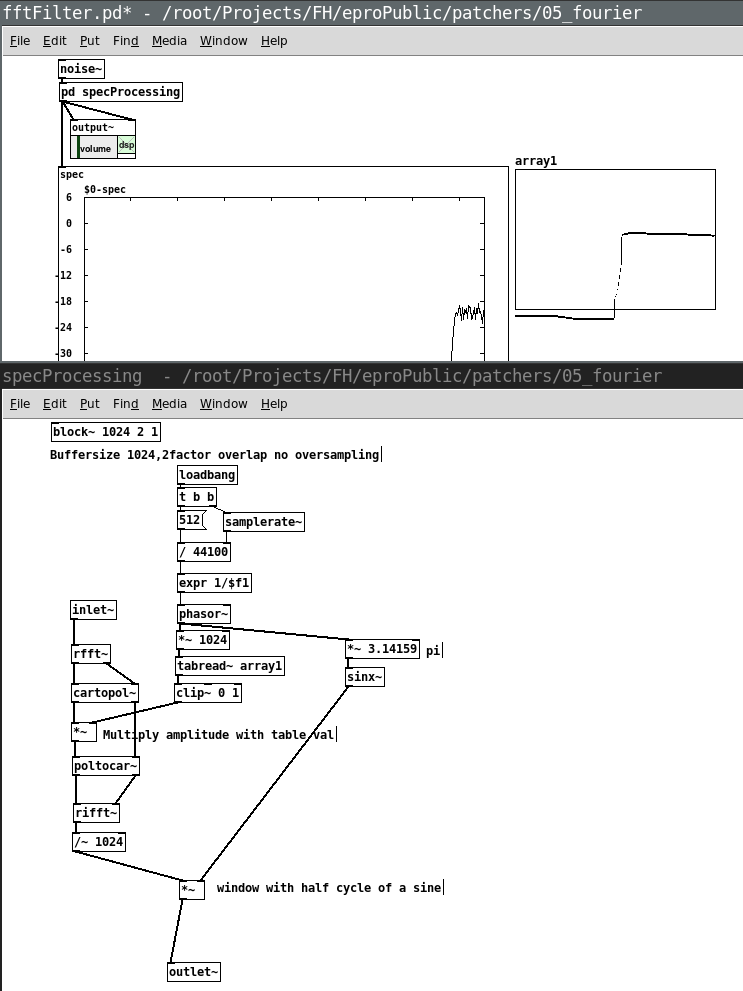
\includegraphics[width = 14cm]{img/spectralFilter2.png}
		\caption{patcher: \texttt{patchers/05\_fourier/fftFilter.pd}}
		\label{fig:spectralFilter}
	\end{center}
\end{figure}
\subsection{Displaying the spectrum}
\begin{figure}[h]
	\begin{center}
		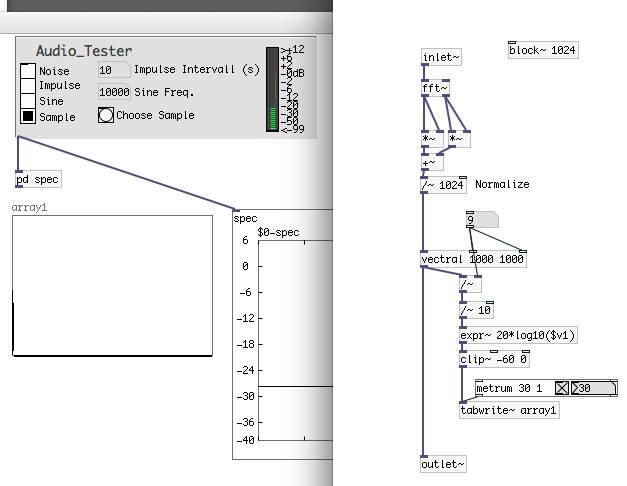
\includegraphics[width = 14cm]{img/showspectrum.png}
		\caption{showspectrum}
		\label{fig:showspectrum}
	\end{center}
\end{figure}

% \subsection{Time Freeze}

